\section{Evaluation}

We conducted a user-centered evaluation of the SensePath tool in order to establish an understanding of its use by an experienced qualitative researcher and to identify opportunities for improvement. To do this we first conducted a number of user studies of participants carrying out an online sensemaking task, and we then recruited an analyst to carry out an analysis of the sensemaking process of the users using SensePath. The process is the same as previous meta observations, with the exception of only using SensePath for the qualitative analysis.

\subsection{Online Sensemaking Task}
In the first part of our study we conducted a number of studies of users performing online sensemaking tasks in order to establish a ground truth dataset for the analyst to use within SensePath. We recruited two participants to take part in this study; a post-doctoral researcher and a PhD student, both male. Participants were given the same task, which was to use Chrome browser to find appropriate accommodation for two academics attending a conference at the World Bank headquarters in Washington, D.C. We provided participants with information about the location and dates of the conference, but gave no further details in the scenario in order to maintain suitable complexity in the task, and to ensure it was as realistic as possible. Both users were given 30 minutes to 	do the sensemaking task, and asked to present us with their choice of hotel and rational behind it at the end. Throughout the study user's interactions and analytic provenance information was collected within SensePath, as well as a screen recording using commercial screen capture software. We also encouraged user's to give think-aloud responses throughout the study, and finally conducted a structured interview asking the user to reveal:

\begin{itemize}
	\item The rationale behind their choice of hotel and information used to support it
	\item The process they went through in order to make their choice of accommodation
	\item Their strategy in approaching the task and the steps they took
\end{itemize}

\subsection{Analysis with SensePath}
For the second part of our evaluation we recruited an analyst to use SensePath to carry out an analysis of the online sensemaking activities collected in the user studies outlined above. We recruited an analyst with 7 years of experience in qualitative research, is the holder of a PhD in an HCI related topic, and has a good understanding of sensemaking. We gave the analyst a short tutorial in the use of the SensePath tool, explaining it's features and use, as well as briefing her on the purpose of the analysis she would carry out. She was provided with a laptop computer running the SensePath tool connected to an external monitor providing a multi-screen set-up as illustrated in \autoref{fig:evaluation-setup}. Both sets of data collected in the previous part of this evaluation were loaded into SensePath, and we asked the analyst to carry out an analysis of each separately. During the analysis, we encouraged the analyst to provide feedback through a think-aloud protocol. We recorded her responses and other observations using written notes. At the end of each analysis we asked the analyst to complete a discovery sheet reporting her findings. The discovery sheet included the following questions:
\begin{itemize}
	\item Identify the steps the user took in choosing suitable accommodation
		\begin{itemize}
			\item The beginning and end of each step in the data
			\item Provide a name (code/theme) for each step
		\end{itemize}
			\item Identify any interesting patterns in the data
			\item Identify the user's strategy in approaching the task, and characteristics which demonstrate this
\end{itemize}

\begin{figure}[ht]
\centering
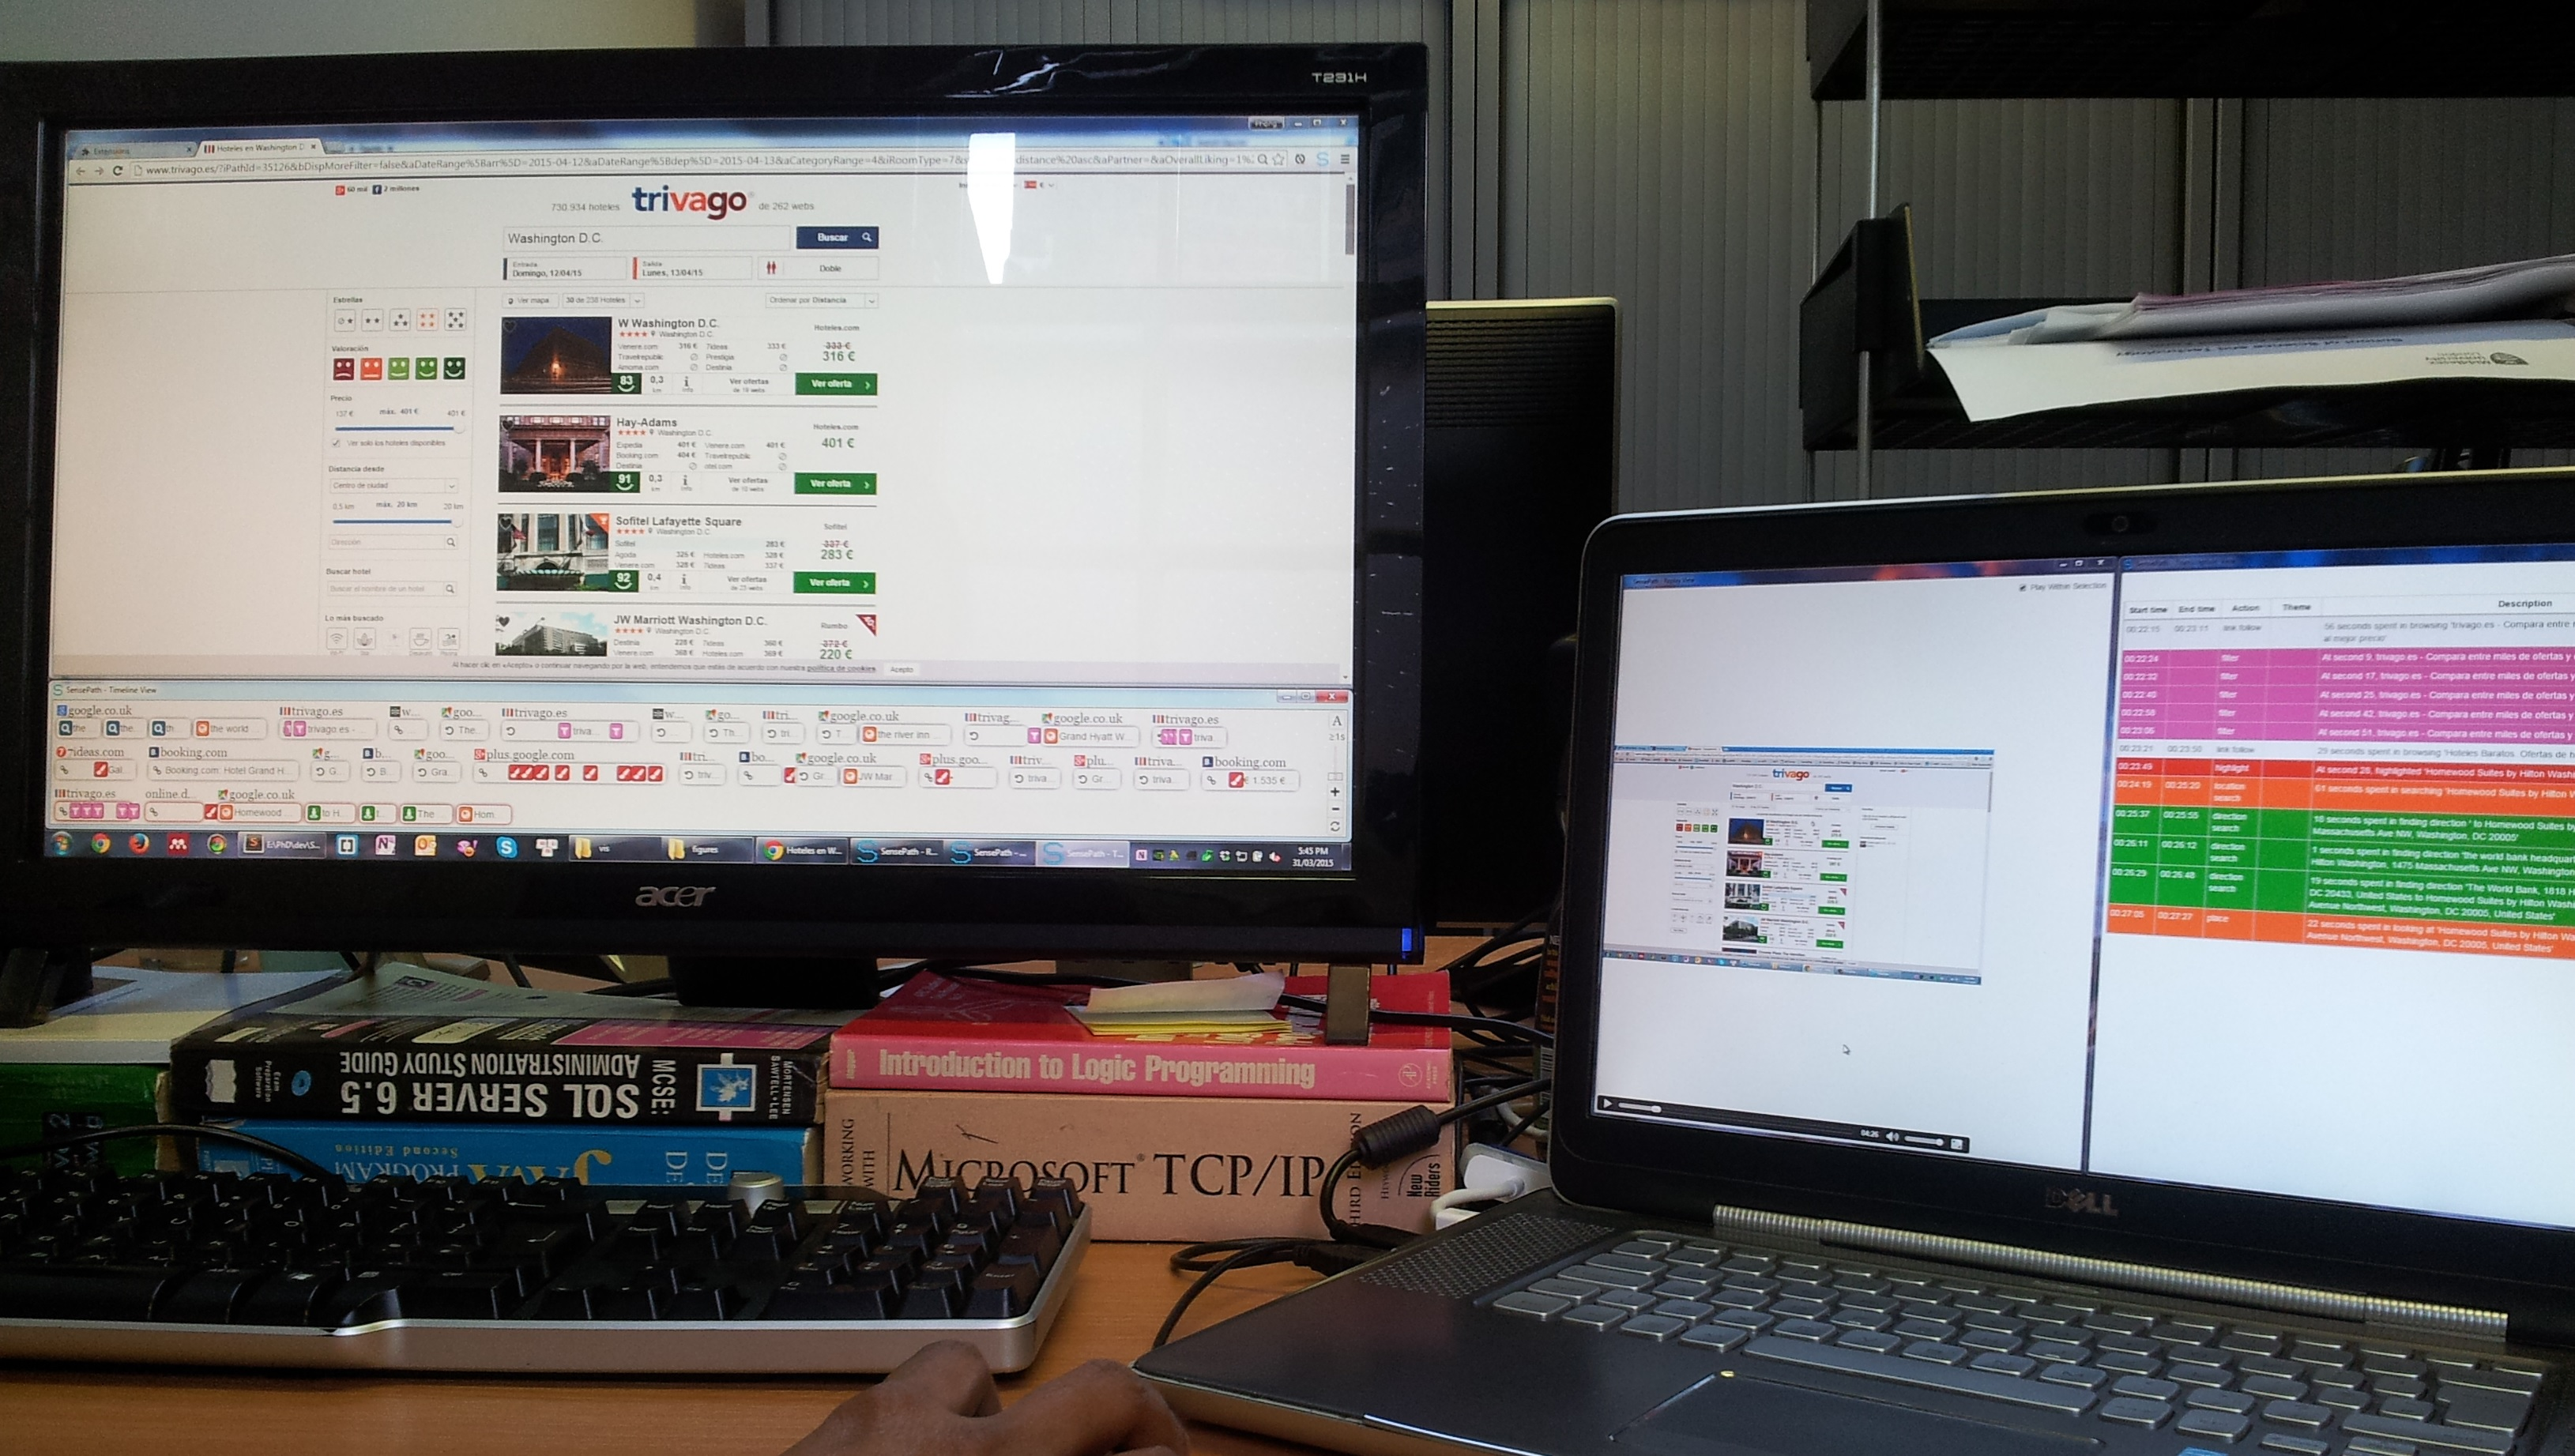
\includegraphics[width=\linewidth]{experiment-setup}
\caption{The setup of the qualitative analysis during evaluation. The monitor on the left shows the timeline and browser view, and the laptop on the right shows the replay and transcription view.}
\label{fig:evaluation-setup}
\end{figure}

\subsection{Findings}
Although the evaluation we have described was of a small scale, and involving the participation of only one analyst, we have yielded some interesting and insightful findings.

The analyst took approximately 1 hour to analyze 30 minutes of study data. This shows a reduction of half the time taken when analyzing study data using SensePath compared with traditional methods of video analysis, which would typically take around 4 hours of analysis for every hour of study data\cite{burr2006vaca}.

The analyst initially used the timeline visualization to see user interactions at a low resolution, before focusing on interesting parts of the data in more detail. As user actions are visualized in a single view, at a high level, the analyst reported that she could quickly make an initial summary assessment of the user's overall performance of the task, before identifying potentially interesting user behaviors in the data which she wanted to look at in further detail. One such example of this is when she saw many highlighting actions on a Google Plus page, next to each other in the timeline, she said ``it seems that the guy [the user performing the task] found interesting information on that [Google Plus] page because he highlighted a lot there''. She then moved the mouse over the action icons to read the highlighted text in the tooltips. Interestingly, she quickly concluded that ``he only focused on negative reviews''. She clicked on some of those icons to open up the Google Plus page to gain more context. Unfortunately, that page is content-dynamic, thus some highlighted texts failed to be reselected. She watched the video in the replay view and heard that the participant was talking to us about his preference to negative reviews (we used think-aloud protocol), which confirmed her initial judgment. She also mentioned that offering highlighting feature to the user seemed useful because it allows the analyst to quickly identify the user's interests.

To understand the whole process, the analyst quickly went through all the actions shown in the timeline. The analyst was able to successfully describe the steps taken by the users in their approach to the task. Those steps are all correct according to our assessment when re-watching the screen capture video and think-aloud recording of the user's sensemaking session. \autoref{fig:evaluation-diagram} shows a reproduction of a written diagram created by the analyst illustrating those steps she identified. As an example of those steps, the analyst pointed to her diagram and explained ``that guy searched for the address of the headquarters, then viewed it in Google Maps to get a sense of where it is''.

\begin{figure}[ht]
\centering
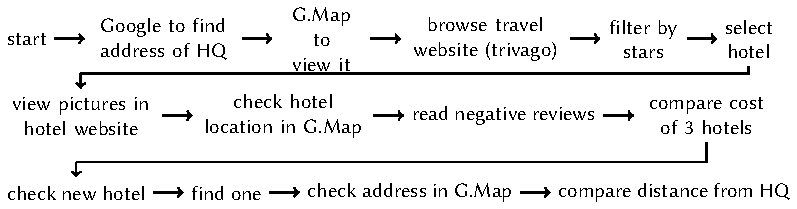
\includegraphics[width=\linewidth]{diagram}
\caption{A reproduction of diagram produced by the analyst during the evaluation illustrating the steps taken by the user in the task.}
\label{fig:evaluation-diagram}
\end{figure}

The analyst reported that using the timeline view she could easily identify interesting recurring patterns in user behavior because all actions are shown together. One such pattern is that when the user finds a hotel in a booking website, he looks at its pictures first, then finds its location in Google Maps, and checks the distance from the headquarters. The analyst stated that the user repeated this pattern for several hotels he found.

The analyst managed to find the rough strategy that the user applied in approaching the task: the user targeted reasonably cheap hotels, evidenced by filtered out 5 stars, but also considered close distance to the headquarters, based on comparison of those hotels in Google Maps. This confirmed with what the user told us: as a professional academic, he did not want to spend too much money from the university.

The analyst commented that the video and audio recordings were intrinsic to carry out a fuller, more detailed analysis by providing additional information that was not available in the timeline and browser views such as the movement of the cursor or scrolling on a page. Therefore, the analyst mentioned that the replay view helped her gain further insight into user behavior. As the analyst did not have to watch the video entirely, she felt that she could save valuable time in the analysis. Furthermore, she stated that as clicking on an action in the timeline view skipped to the relevant place in the screen capture, further time was saved in scrubbing through the video, which often happened in her experience of analyzing video data. One such example of using the replay view is when she saw a long action bar with location search icon. She knew that the user spent a lot of time in a Google Maps page, looking at a specific location; however, what exactly he was doing is neither available in the timeline nor the browser view. Thus, she needed to watch the video to get more information.

\subsubsection{Opportunities for further development}
Overall our tool proved to be useful in enabling an analyst to gain insights into a user's online sensemaking process quickly and much less costly than a traditional qualitative analysis. In our analysis however we were able to identify opportunities for further design and development of SensePath. Foremost, though the analyst was able to quickly become familiar with the tool, she found it difficult to find the start time and end time of user actions in the timeline view in the absence of a visible scale. Also, although the tool is able to capture and visualize actions such as filtering, the analyst felt that she needed to refer to the video and audio recordings to find what filters or sorting the user performed, as this was not apparent in SensePath. This meant she needed to refer to video and audio data to try and find this.